\documentclass[a4paper,12pt,twoside,titlepage]{article}

%Additional packages
\usepackage[utf8]{inputenc}
\usepackage[T1]{fontenc}
\usepackage[dutch,english]{babel}
\usepackage{syntonly}
\usepackage[official]{eurosym}
\usepackage{csquotes}

% Handle images
\usepackage{graphicx}
\graphicspath{ {./images/}{./styles/} }
\usepackage{float}
\usepackage{wrapfig}

% Handle URLs
\usepackage{xurl}
\usepackage{hyperref}
\hypersetup{colorlinks=true, linkcolor=blue, citecolor=blue, filecolor=blue, urlcolor=blue, pdftitle=, pdfauthor=, pdfsubject=, pdfkeywords=}

% Tables and listings
\usepackage{multirow,tabularx}
\usepackage[table]{xcolor} % Table colors
\usepackage{scrextend}
\addtokomafont{labelinglabel}{\sffamily}
\usepackage{listings}
\usepackage{adjustbox}

% Turn on indexing
\usepackage{imakeidx}
\makeindex[intoc]

% Define colors
\usepackage{color}
\definecolor{ashgrey}{rgb}{0.7, 0.75, 0.71}




% Listing style
\lstset{
  backgroundcolor=\color{ashgrey}, % choose the background color; you must add \usepackage{color} or \usepackage{xcolor}; should come as last argument
  rulecolor=\color{black},         % if not set, the frame-color may be changed on line-breaks within not-black text (e.g. comments (green here))
  frame=single,	                   % adds a frame around the code
  basicstyle=\footnotesize\ttfamily,  	   % the size of the fonts that are used for the code
  extendedchars=true,    	   % lets you use non-ASCII characters; for 8-bits encodings only, does not work with UTF-8
  breakatwhitespace=true, 	   % sets if automatic breaks should only happen at whitespace
  breaklines=true,        	   % sets automatic line breaking
  keepspaces=true,        	   % keeps spaces in text, useful for keeping indentation of code (possibly needs columns=flexible)
  columns=fullflexible,	  	   % Make sure no extra spaces are added.
  showstringspaces=false, 	   % if true show spaces in strings adding particular underscores
  showspaces=false        	   % show spaces everywhere adding particular underscores; it overrides 'showstringspaces'
}



% Uncomment for production
% \syntaxonly

% Style
\pagestyle{headings}

% Define document
\author{D. Leeuw}
\title{Python}
\date{\today\\
0.0.0
\vfill
\raggedright
\copyright\ 2025 Dennis Leeuw\\

%\begin{figure}

\includegraphics[width=0.3\textwidth]{CC-BY-SA-NC.png}
%\end{figure}

Dit werk is uitgegeven onder de Creative Commons BY-NC-SA Licentie en laat anderen toe het werk te kopi\"eren, distribueren, vertonen, op te voeren, en om afgeleid materiaal te maken, zolang de auteurs en uitgever worden vermeld als maker van het werk, het werk niet commercieel gebruikt wordt en afgeleide werken onder identieke voorwaarden worden verspreid.


}


\begin{document}
\selectlanguage{dutch}

\maketitle

%%%%%%%%%%%%%%%%%%%
%%% Introductie %%%
%%%%%%%%%%%%%%%%%%%

%%%%%%%%%%%%%%%%%
%%% De inhoud %%%
%%%%%%%%%%%%%%%%%

% requires: 
% provides: programmeren, python
\section{Wat is Python?}
Python is een programmeertaal\index{programmeertaal}. Met een programmeertaal kan je een computer dingen voor je laten doen. Doordat de computer dan werk voor je doet kan jij andere dingen doen (nee, niet gamen). Tijdens het programmeren\index{programmeren} gebruik je een programmeertaal om programma-code\index{programma-code} of kortweg code\index{code} te schrijven. De programma-code schrijf je in een tekst-bestand zonder opmaak, we gebruiken daarom geen Word om een computer programma te schrijven maar een editor\index{editor}. Een editor is een heel simpele tekstverwerker zonder alle speciale functies als het invoegen van plaatjes, het nummeren van pagina's of het maken van hoofdstuk-koppen. De meeste programmeurs gebruiken een IDE\index{IDE} (Integrated Development Environment\index{Integrated Development Environment}).

Er zijn verschillende talen om een computer te vertellen wat hij moet doen. Python is er daar \'e\'en van. Programmeertalen kunnen grofweg in twee soorten verdeeld worden. We hebben de scripting-talen\index{scripting} en de talen die eerst gecompileerd\index{gecompileerd} moeten worden.

Talen die eerst gecompileerd moeten worden worden ook geschreven in een editor of een IDE, maar nadat het programma geschreven is gaat deze eerst door een compiler\index{compiler}. Deze compiler maakt van de programma-code een binary\index{binary}. Op Windows systemen is dit vaak een bestand met de extensie .exe van executable\index{executable}. Een executable is een programma dat direct door een computer uitgevoerd kan worden. De binary bevat 1-en en 0-en die direct door de computer begrepen worden. Een executable kan dan ook op elke computer, met dezelfde processor en hetzelfde operating system, uitgevoerd worden zonder dat de programma-code aanwezig is.

Scripting talen hebben geen compiler, maar een interpreter\index{interpreter}. De taal waarin het programma is geschreven wordt op de computer door de interpreter omgezet naar machinetaal\index{machinetaal}, of wel de 1-en en 0-en, om dan uitgevoerd te worden. Op elke computer waarop je het programma wilt draaien moet dus een interpreter en de code aanwezig zijn om de code te kunnen uitvoeren.

Python is een scriptingtaal en heeft dus een Python-interpreter nodig om gebruikt te kunnen worden.

\subsection{Opdrachten}
\begin{enumerate}
\item Zoek op Internet naar 3 programmeertalen die gecompileerd moeten worden en welke compiler daarvoor gebruikt kan worden
\item Zoek op Internet naar 3 programmeertalen die net als Python ook scripting-talen zijn en welke interpreter daarvoor nodig is
\item Zijn compilers en interpreters binaries? Leg je antwoord uit.
\end{enumerate}


\section{Installatie van de Python-interpreter}
\subsection{Windows}
Volg de instructies op \url{https://learn.microsoft.com/en-us/windows/python/scripting} om Python te installeren. Alleen het kopje \textquote{Install Python}. Je installeert nu de Python-interpreter.

Als Python ge\"installeerd is kan je via de zoekbalk Python opzoeken en opstarten, zoals je kan zien in \ref{fig:pythonint}

\begin{figure}[H]
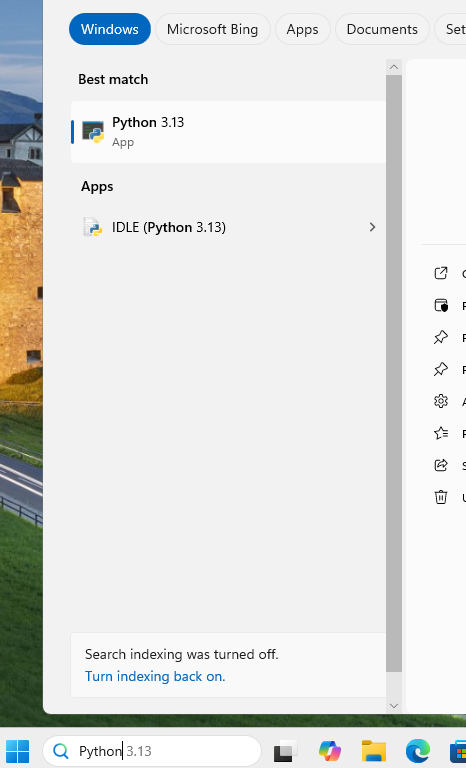
\includegraphics[width=0.9\textwidth]{Screenshot-Python-Start-Selection.png}
        \caption{Zoek en start Python}
        \label{fig:pythonint}
\end{figure}

Om de Python-interpreter af te sluiten type je \texttt{exit()}. Denk om de haakjes aan het einde.


\section{Hello World!}
De meeste programmeertalen beginnen bij hun uitleg over de taal met het op het scherm printen van de tekst \textquote{Hello World!}, laten wij voor deze Python lessen daar ook maar mee beginnen. Python maakt gebruik van een interpreter en dus kunnen we de interpreter opstarten en daar het commando intypen. Start Python op door op de command line \texttt{python} te typen en enter te geven.
\begin{lstlisting}[language=python]
Python 3.11.2 (main, Apr 28 2025, 14:11:48) [GCC 12.2.0] on linux
Type "help", "copyright", "credits" or "license" for more information.
>>> print("Hello World!")
Hello World!
>>> exit()
\end{lstlisting}
De \textgreater\textgreater\textgreater geeft aan dat je op de Python prompt zit. Na deze drie groter dan tekens mag je python code intypen. In ons geval bestaat de opdracht aan Python uit het commando \texttt{print()} met tussen quotes de tekst die we op het scherm afgebeeld willen zien. Na de enter zal Python direct de tekst laten zien. Met het commando \texttt{exit()} verlaten we de interpreter.

We kunnen ook een tekstbestand maken in onze editor met daarin het commando:
\begin{lstlisting}[language=python]
print("Hello World!")
\end{lstlisting}
Als we dit document opslaan met een \texttt{.py} extensie, bijvoorbeeld als \texttt{hello.py} dan kunnen we dit script door python laten uitvoeren door het script als argument mee te geven aan \texttt{python}:
\begin{lstlisting}[language=python]
python hello.py
\end{lstlisting}

Het uitvoeren van commando's direct in de interpreter is makkelijk om zaken te testen, maar om dingen ook voor de toekomst veilig te stellen is het beter om scripts te gebruiken zodat scripts die je een keer gemaakt hebt ook later weer kunt gebruiken.



\section{IDE}
Een Integrated Development Environment\index{Integrated Development Environment}\index{IDE} is meer dan een code editor. Een IDE helpt je bij het schrijven van code door syntax-highlighting, code aanvullingen en waarschuwingen als je iets schrijft dat tegen de regels (syntax) is. Ook een vast onderdeel van een IDE is de mogelijkheid om je code snel te testen met vaak ook opties om dat bijvoorbeeld stap voor stap te doen, zodat je makkelijker kan zien op welke regel het fout gaat.


\subsection{Windows: Visual Studio Code}
\begin{itemize}
\item Zoek in de Windows Store op Visual Studio Code en installeer deze
\item Installeer de Python extension voor Visual Studio Code
\item Start PowerShell en run:
\begin{lstlisting}[language=bash]
python.exe -m pip install --upgrade pip
\end{lstlisting}
\end{itemize}

\subsection{Linux: Visual Studio Code}
\begin{itemize}
\item Download je linux versie van https://code.visualstudio.com/
\item Voor .deb doe:
\begin{lstlisting}[language=bash]
sudo dpkg -i ~/Downloads/ode_1.101.0-1749655245_amd64.deb # Vervang het versienummer met jouw versie
\end{lstlisting}
Voor .rpm doe:
\begin{lstlisting}[language=bash]
sudo rpm -i ~/Downloads/ode_1.101.0-1749655245_amd64.rpm # Vervang het versienummer met jouw versie
\end{lstlisting}
\item Sta Microsoft toe om de applictie toe te voegen aan de package database
\end{itemize}


%\subsection{PyCharm}
%\begin{itemize}
\item Ga naar \url{https://www.jetbrains.com/pycharm/} en download PyCharm
\item mkdir -p ~/Apps
\item cd ~/Apps
\item tar zxvf ~/Downloads/pycharm-2025.1.2.tar.gz # Vervang versienummer met jouw versie
\item cd pycharm-2025.1.2/bin # Let ook hier op het versienummer
\item ./pycharm.sh
\end{itemize}


%%%%%%%%%%%%%%%%%%%%%
%%% Index and End %%%
%%%%%%%%%%%%%%%%%%%%%
\printindex
\end{document}

%%% Last line %%%
